%% FEL CVUT

\documentclass[journal]{IEEEtran}
\usepackage{graphicx}


\begin{document}
%
% paper title
\title{Multi-Agent Systems Using Kobuki Turtlebots:\\Leader-Follower Premise}
\author{Sinchiguano Cesar}


\markboth{Intelligent and Mobile Robotics Group, Czech Technical University in Prague, 20018/19}{Shell \MakeLowercase{\textit{et al.}}: Bare Demo of IEEEtran.cls for Journals}
\maketitle

%done
\begin{abstract}

%%%%%%%%%%%%%%%%%
Multi-agent system is a topic that has generated a lot interest in the research community. This interest is because a multi-agent systems present a more robust and cheaper solution to a certain tasks that are better performed using several low-cost robots rather than a single one. Multi-agent system can be achieved through many approaches. The approach used in this paper is the one based on the leader-follower premise.
\end{abstract}


\section{Introduction}

%%%%%%%%%%%%%%%%%%%%%%%%%%%%%%%

Multi-robot systems present a more robust and cheaper solution to certain tasks that are better performed using several low-cost robots rather than a single one. This gives rise to the formation control problem. The formation problem has been regarded as an important problem in multi-robot systems where the goal is to make a fleet of autonomous mobile robots move toward and maintain a desired geometric shape. According to the survey presented in (Guanghua et al., 2013), and the references therein, formation structure can be divided into three strategies: the leader–follower strategy, the behavioural and the virtual structure approaches. Several approaches have been proposed in the literature to solve this problem. However, most of the existing literature tackle the theoretical side of the problem mainly the controller design. Nevertheless, some of them have carried on real experiments to prove the effectiveness of their proposed controller. 

In this paper, we propose the use of ROS as a new framework so that real experiments for the formation control problem can be conducted effectively. Due to its simplicity and scalability, the leader-follower approach is considered in this paper also. However, the proposed framework can be extended so that other formation strategies or consensus algorithm can be implemented. 
The rest of this paper will be organized as follow: The introduction about ROS concepts is highlighted in Section II, with the software setup in Section III, followed by a detailed explanation of the software processes and the needed ROS packages are presented  in Section IV, finally conclusions drawn from this experiment and some future work directions in Section VI



\begin{figure}[!h]
\begin{center}
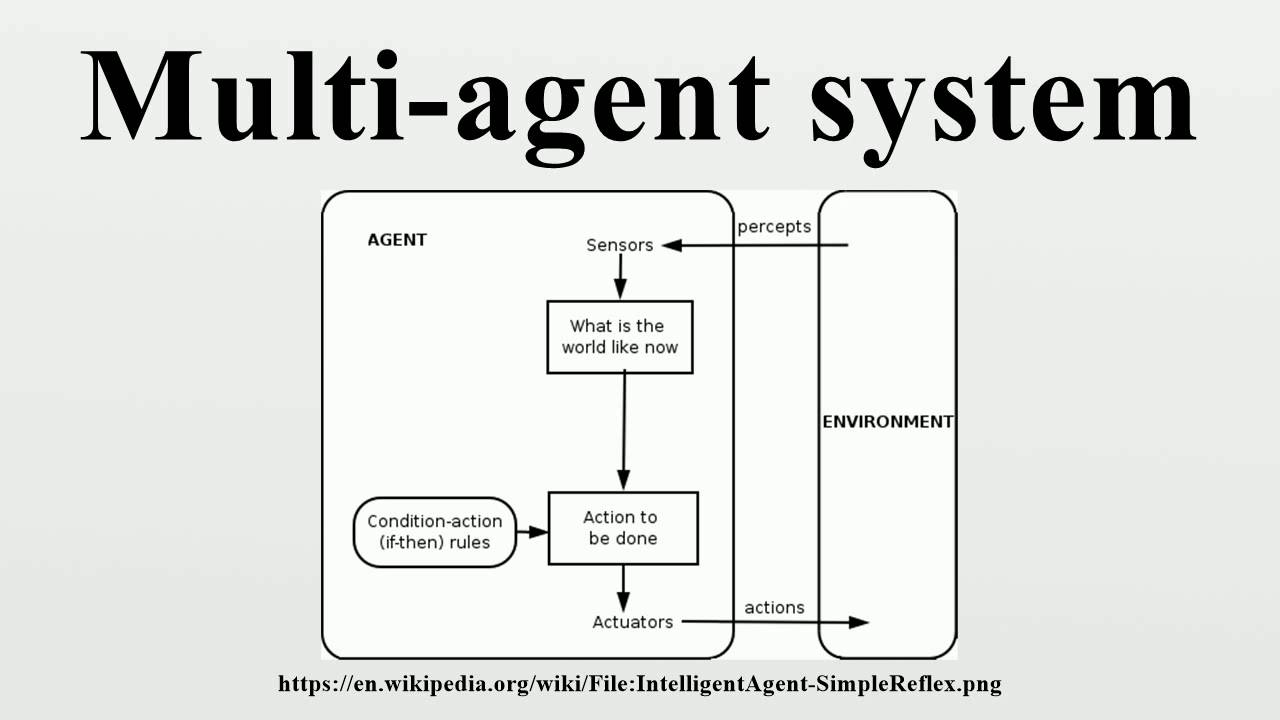
\includegraphics[width=2in]{one.jpg}
\caption{An example of multi-agent system. \cite{temp1}}
\end{center}
\label{fig:mypicture1}
\end{figure}


%%%%%%%%%%%%%%%%%%%%%%


\begin{enumerate}
\item \textbf{.......}



%%%%%%%%%%%%%%%%%%%%%%
%%%%%%%%%%%%%%%%%%%%%%
\item \textbf{....}


\end{enumerate}

%%%%%%%%%%%%%%%%%%%%%%%%%%%%%
%%%%%%%%%%%%%%%%%%%%%%%%%%%%%%%


\section{Backgroung}
%done
\begin{enumerate}
\item \textbf{Robotic Operating System (ROS)}\\
ROS is a flexible framework for writing robot software. It is a collection of tools, libraries, and conventions that aim to simplify the task of creating complex and robust robot behaviour across a wide variety of robotic platforms . It is based on the concepts of nodes, topics, messages and services. A node is an executable program that performs computation. Nodes need to communicate with each other to complete the whole task. The communicated data are called messages. ROS provides an easy way for passing messages and establishing communication links between nodes, which are running independently. They pass these messages to each other over a Topic, which is a simple string. However, topics are asynchronous, synchronous communication is provided by services. Services act in a call-response manner where one node requests that another node execute a one-time computation and provide a response. For more details about ROS, the reader can refer to \cite{temp2}.



\item \textbf{Architecture of the System}\\


\end{enumerate}


%%%%%%%%%%%%%%%%%%%%%%%
%%%%%%%%%%%%%%%%%%%%%%%
%working on
\section{Experimental setup}

The test space consist of two Kobuki TurtleBots. It is a low-cost, open source differential drive robot. It consists of a mobile base, a RGB-D sensor and a CPU making it a good  entry-level mobile robot platform. The Kobuki was chosen because it is an open source UGV (Unmanned ground vehicle) platform, making it perfect for research and development. The Kobuki SDK (Software development kit) is based on ROS, which is the preferred development platform by the Intelligent and Mobile Robotics Group because of its intuitive publisher/subscriber message passing structure that allows robust and simple communication within multiple  facets of a robotic system. The Fig 2 shows two Turtlebot robots which are equipped with Kinect Sensors. The robots run ROS (Robot Operating System), and are supported by various ROS libraries. 

\begin{figure}[!h]
\begin{center}
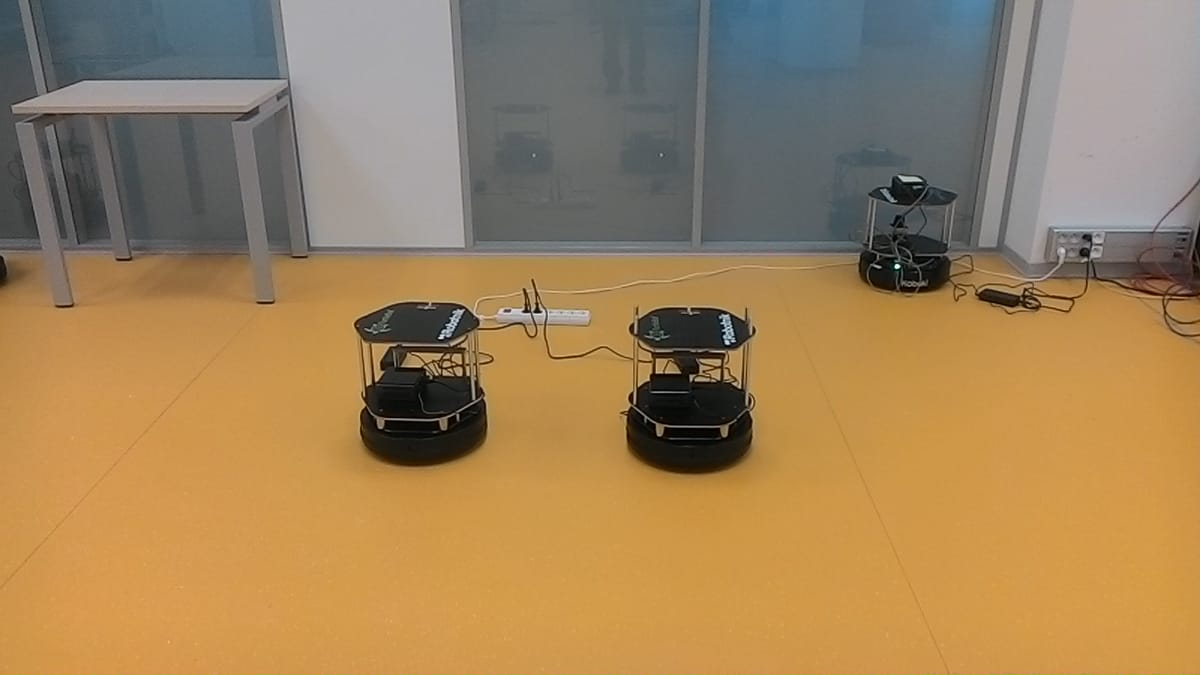
\includegraphics[width=2in]{two.jpg}
\caption{Two turtlebots used in the experimental test bed.}
\end{center}
\label{fig:mypicture2}
\end{figure}








%##################################################
%#################################################

\section{Software Processes}

In addition to the basic nodes called turtlebot{\_}bringup needed for running the robots, four additional nodes are indispensable for controlling the robots to achieve formation. 
The multi{\_}agents node for deploying the Turtlebot robots to work with, the tf{\_}turtle responsible for keeping track of the robot's postures, multi{\_}master node for data transmission and the turtle node that executes the control algorithm. The nodes are running simultaneously and thus they have to communicate to each other through ROS topics or ROS services as depicted in fig.3. Note that on each robot, all the nodes are executed under a specific namespace for the robot. The ROS parameter ‘tf{\_}prefix’ is exclusive for each robot as well.
\begin{figure}[!h]
\begin{center}
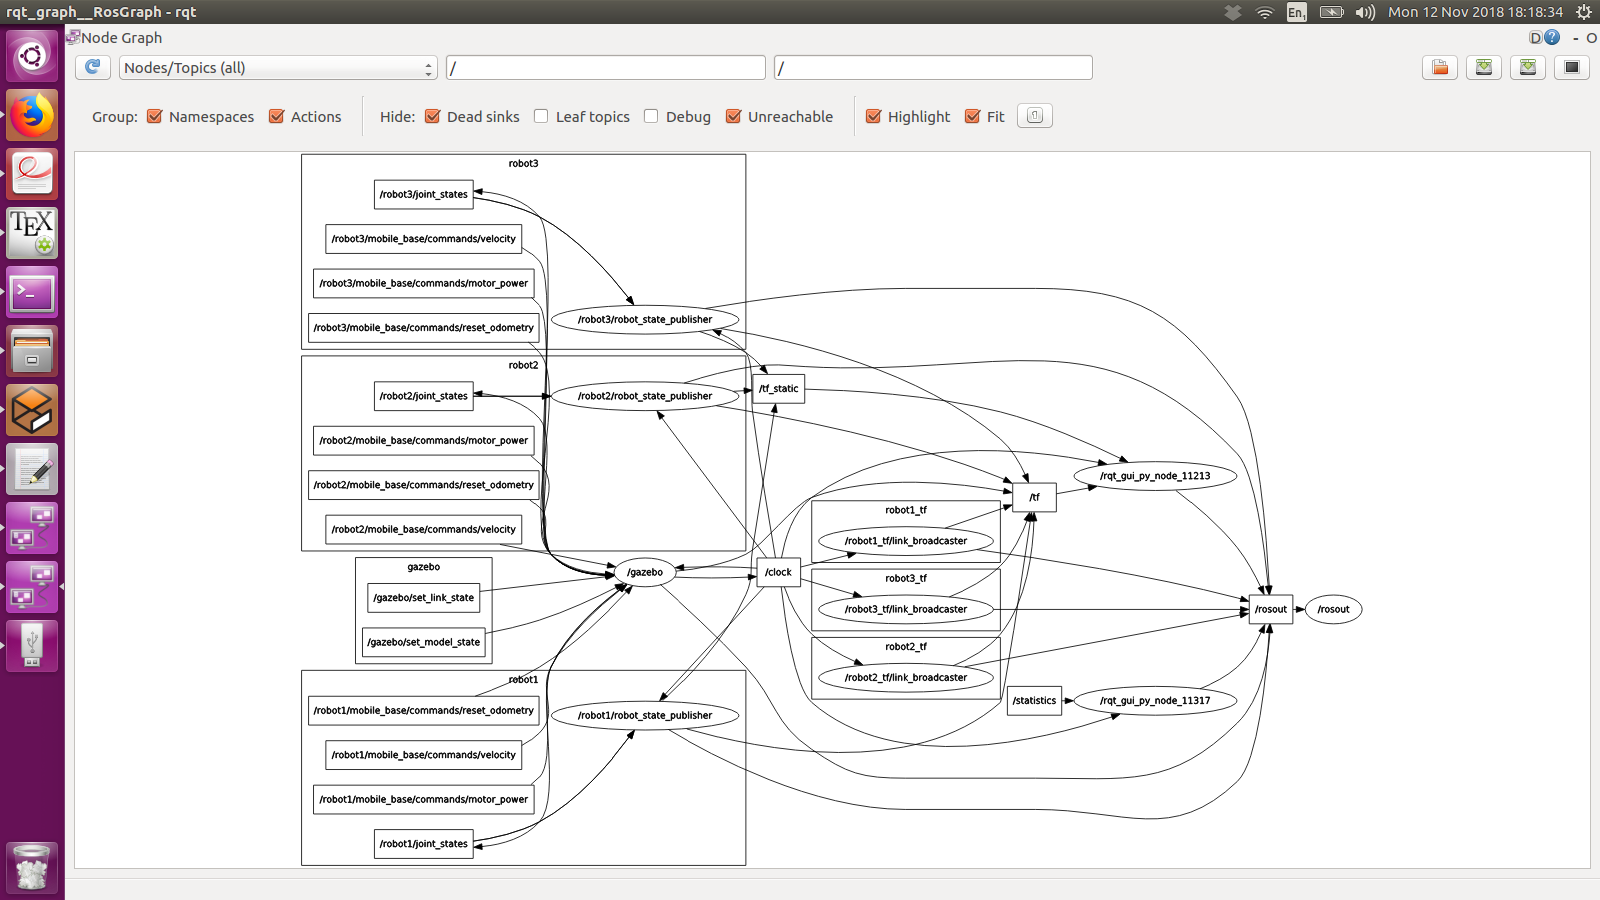
\includegraphics[width=2in]{4.png}
\caption{A rosgraph showing what talks to what.}
\end{center}
\label{fig2:mypicture2}
\end{figure}



\begin{enumerate}
%>>>>>>>>>>>>>>>>>>>>>>>>>>>>>>>>>>>>>>>>>>>>>>
%subtitle.....01
\item \textbf {Simulating Multiple Turtlebots in Gazebo}\\
This is an example of simulating and controlling multiple Turtlebot robots. It is built as an extension of the Simulating Turtlebot tutorial on \cite{temp4}.

\begin{figure}[!h]
\begin{center}
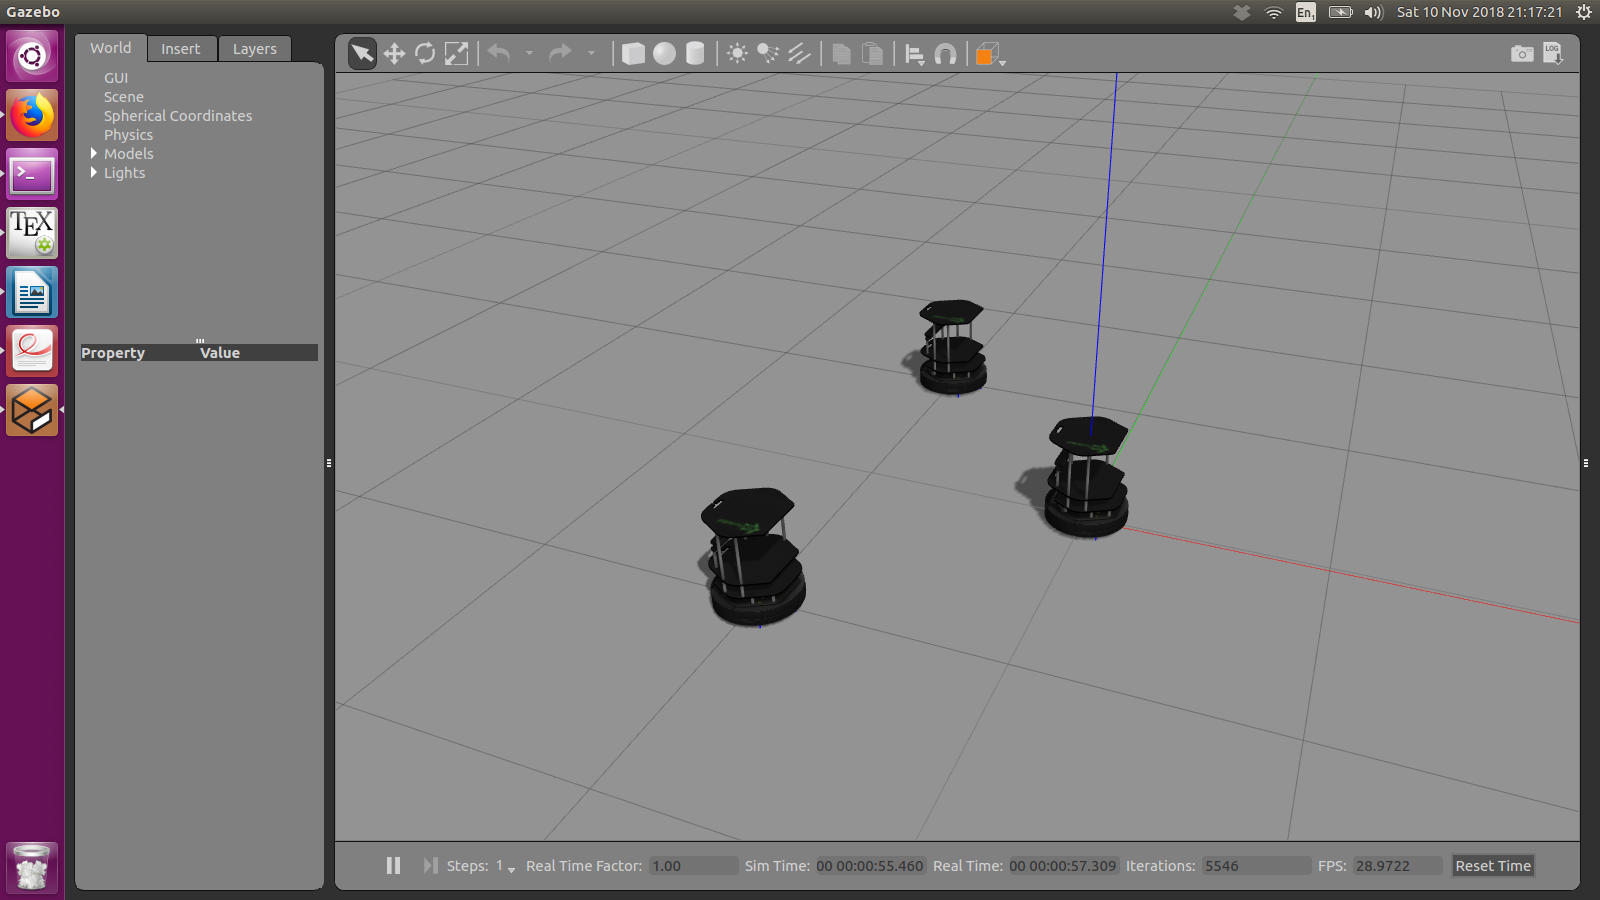
\includegraphics[width=2in]{two.png}
\caption{A general view of the system.}
\end{center}
\label{fig:mypicture3}
\end{figure}

\begin{enumerate}
\item \textbf {Quick Start}

The main.launch file is a working example that instantiates two simulated Turtlebots in Gazebo. 

You will first need to install the following packages in your workstation:
\begin{enumerate}
\item {turtlebot}\cite{temp6}.
\item {kobuki}\cite{temp8}.
\item {turtlebot{\_}simulator}\cite{temp7}.
\item {turtlebot{\_}interactions}\cite{temp9}.
\end{enumerate}
Then after you have these packages in your workspace, place the multi{\_}agents\cite{temp5} package in your src diretory.\\
As long as all of the system dependencies of your packages are installed, we can now build your new packages.\\
In a catkin workspace

\begin{enumerate}
\item {{\$} catkin{\_}make}.
\end{enumerate}

Before continuing source your new setup.*sh file:
\begin{enumerate}
\item {{\$} source devel/setup.bash}.
\end{enumerate}

To make sure your workspace is properly overlayed by the setup script, make sure ROS{\_}PACKAGE{\_}PATH environment variable includes the directory you are in with the following command:

{\$} echo {\$}ROS{\_}PACKAGE{\_}PATH



%%%%%%%%%%%%%%%%%%%%%%%%%%%%%%%%%%%%%%%%%%%%%%%
\item \textbf {Description: multi{\_}agents package}


If everything was done with the commands above then it should just work. From there, to learn what it does, I woud recommend going over the multi{\_}agent.launch, one{\_}turle.launch and main.launch files those who can be located inside your catkin{\_}ws with the following command:\\
{\$} cd src/multi{\_}agents/launch \\
which will lead you to the launch files mentioned above. All of them are binding one another. The only one that it should be launched is the one named as main.launch file which does the heavy lifting of setting up each Turtlebot. Here is a high-level outline of what this package does.

main.launch:
\begin{enumerate}
\item {Starts Gazebo (both the sim engine and the gui)}
\item {Start some visualization and debugging tools (rviz,rqt{\_}console, etc.)}
\item {multi{\_}agents.launch}

\begin{enumerate}
\item {Accept namespace and initial pose arguments from one{\_}turtle.launch}.
\item {Set the tf{\_}prefix based on the namespace}
\item {Call a xacro robot{\_}description with namespace and tf{\_}prefix arguments}
\item {Spawn the Turtlebot model in Gazebo using gazebo{\_}ros}
\item {Start a robot{\_}state{\_}publiser node}
\end{enumerate}
\end{enumerate}
Here are some screen captures and images to illustrate what you should see if things are working properly.
    
 

Four Turtlebot robots in Gazebo
\begin{figure}[!h]
\begin{center}
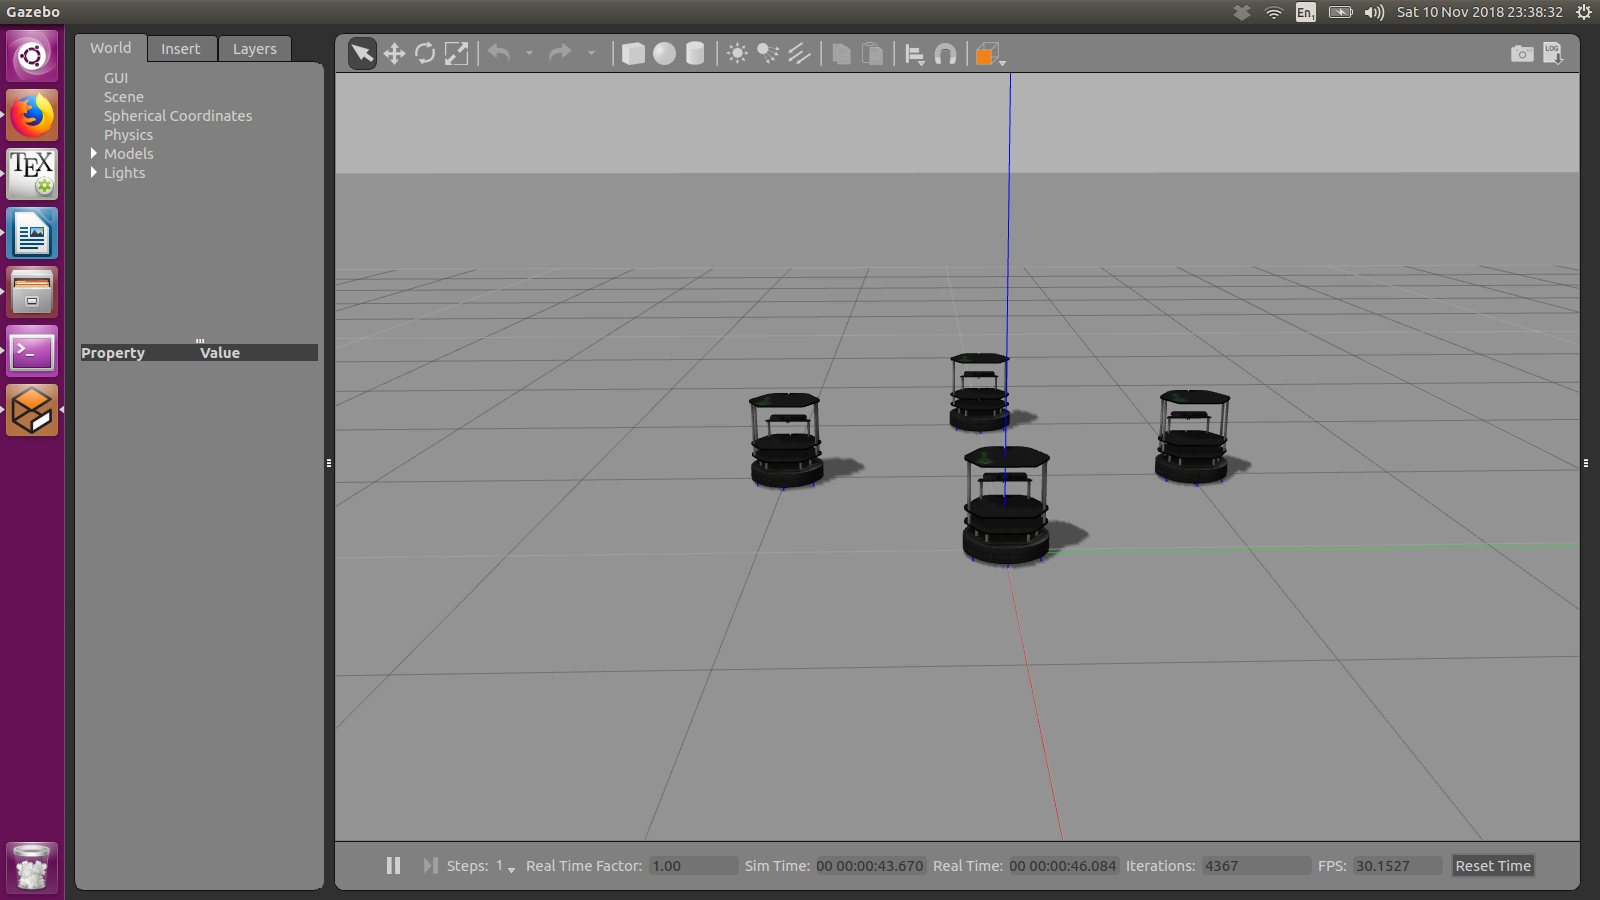
\includegraphics[width=2in]{three.png}
\caption{A general view of the system with four multi-agents.}
\end{center}
\label{fig:mypicture4}
\end{figure}


\end{enumerate}



%>>>>>>>>>>>>>>>>>>>>>>>>>>>>>>>>>>>>>>>>>>>>>>
%subtitle.....02
\item \textbf {Transform}

When doing tasks with a robot it is crucial that the robot be
aware of where it is itself as well as where the rest of the world
is in relation to itself. For the leader-follower premise each robot takes another neighboring robot as a leader to determine its motion so that for the control laws proposed in this paper show that the leader’s relative coordinates and velocities are needed in the control laws implemented on the followers. The package called tf{\_}turtle will deal with it. It will start a static{\_}transform{\_}publisher node to establish the tf transfrom from the world to the specific odometry frame e.g robot2{\_}tf/odom.

\begin{figure}[!h]
\begin{center}
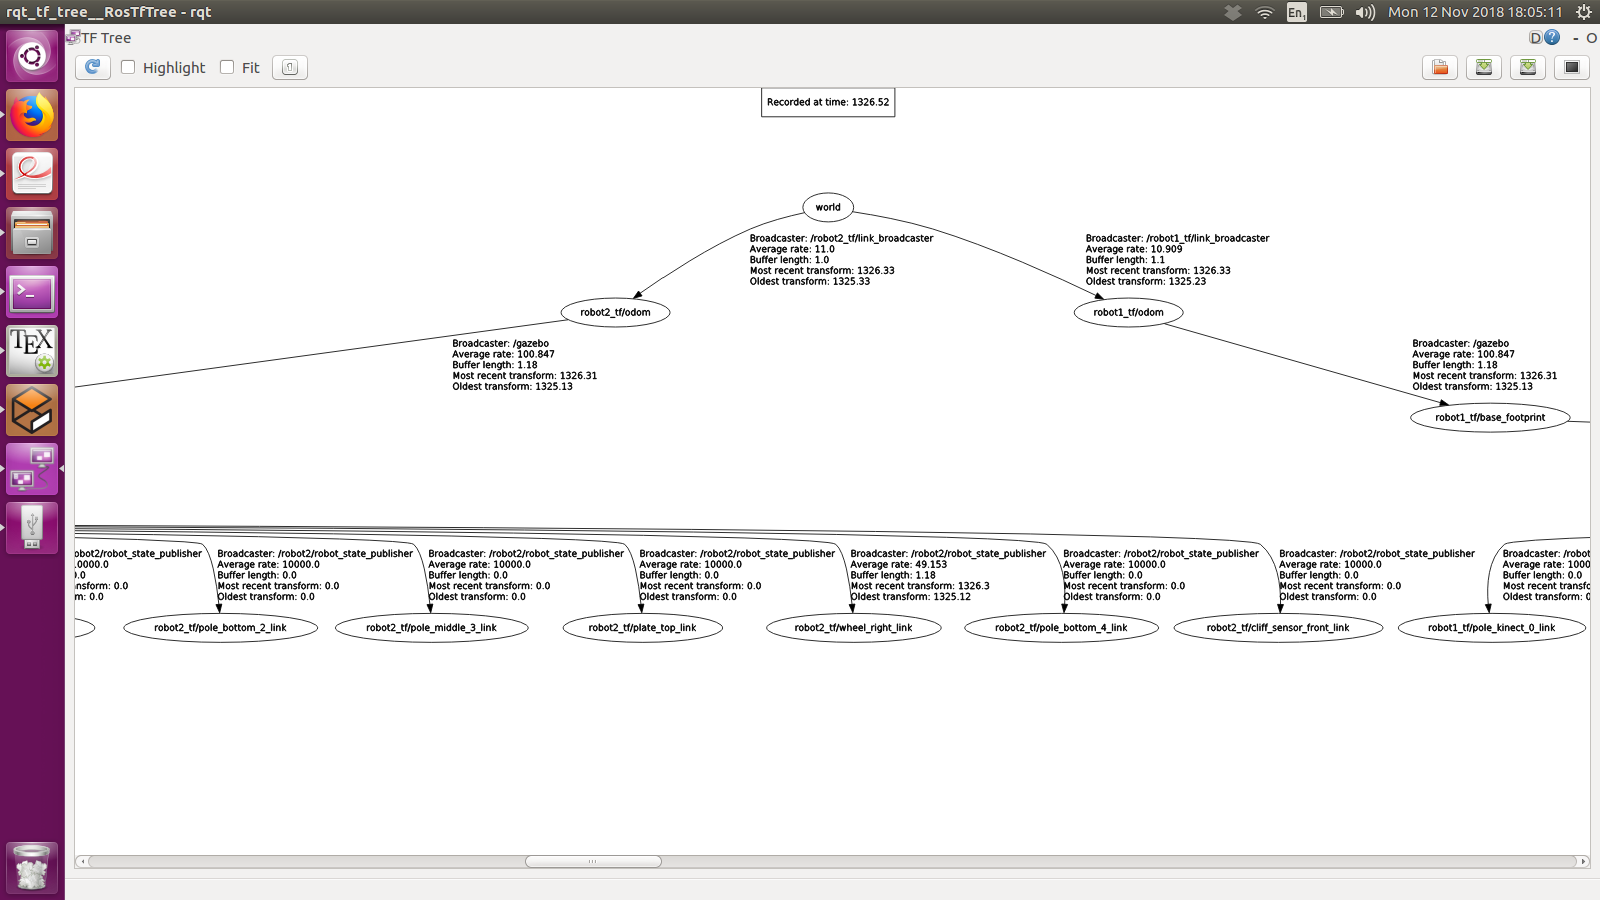
\includegraphics[width=2in]{3.png}
\caption{View from rqt{\_}tf{\_}tree of the tf arrangement.}
\end{center}
\label{fig:mypicture4}
\end{figure}


\begin{enumerate}
\item \textbf {Quick Start}\\
The robot{\_}1.launch file is a working example that initialize the transform node for two Turtlebot robots.
You will first need to install the following packages in your workstation:
\begin{enumerate}
\item {geometry}\cite{temp10}.

\end{enumerate}

Then after you have these packages in your workspace, place the tf{\_}turtle\cite{temp11} package in your src diretory.\\
As long as all of the system dependencies of your packages are installed, we can now build your new package.\\
In a catkin workspace
\begin{enumerate} 
\item {{\$} catkin{\_}make}.
\end{enumerate}

Before continuing source your new setup.*sh file:
\begin{enumerate}
\item {{\$} source devel/setup.bash}.
\end{enumerate}

\end{enumerate}








%subtitle.....03
\item \textbf {Communication data}\\
A robust communication between the Turtlebot robots is needed in order to transmit the leader’s postures and velocities to its follower. These data are essential for controlling the follower to keep the desired separation and bearing with the leader. The leader-follower premise is implemented using two methods: (1)Single-master system, and (2)multi-master system. The methods aforementioned make use of the distributed computing and communication architecture of the Robot Operating System (ROS). The detail of each implementation and their respective use are presented next in this section. 

\begin{enumerate} 
\item \textbf {Single Master System}\\

In a single master system, ROSCORE runs on one machine
which is called the master. Other nodes work in a distributed similar fashion on different machines. The nodes can run anywhere on the network except the driver nodes, which runs on the system that is directly connected to the hardware. All the nodes need to connect to the master. They connect via ROS{\_}MASTER{\_}URI which can be set in .bashrc file of the respective machines as shown below. All the machines in the network have a bidirectional connection with each other. Also, the host IP and the master IP will be same in case of the master machine.


\begin{enumerate}
\item \textbf {Quick Start}\\
The following commands are required to be executed to activate the single master system:
\textbf{For computer one (turtlebot@turtle01)}.
export ROS{\_}MASTER{\_}URI=http://10.37.2.152 :11311\\
export ROS{\_}IP=10.37.2.152\\
\textbf{For computer two (turtlebot@turtle02)}.
export ROS{\_}MASTER{\_}URI=http://10.37.2.152 :11311\\
export ROS{\_}IP=10.37.2.243
\end{enumerate}
For more details about NetworkSetup the reader to should refer to the ROS/NetworkSetup \cite{temp11}


\item \textbf {Multi Master System}

Many of the limitations of a single master system can
be overcome by having multiple masters running their own
independent roscore. This makes
the system robust as the failure of one will not lead to the
failure of the complete system. Since the visibility of topics is
limited to the scope of each roscore environment, there are
no namespace conflict with topics in a multi-master system.

To implement a multi-master System, a package called
multimaster{\_}fkie is needed [12] and is already installed from source in each one of the Turtlebot. This allows two important pro-cesses, master{\_}discovery and master{\_}sync to run
simultaneously. The function of master{\_}discovery is to
send multicast messages to the network so that all roscore
environments become aware of each other. The other process called master{\_}sync enables us to select which topics can shared between different roscore. Without master{\_}sync node, no information can be accessed by other roscores. 

\begin{enumerate}
\item \textbf {Quick Start}\\
The following commands are required to be executed to activate multi-master mode in each machine.

\textbf{For computer one (turtlebot@turtle01)}.
export ROS{\_}MASTER{\_}URI=http://localhost :11311\\
export ROS{\_}IP=10.37.2.152\\
rosrun master{\_}discovery{\_}fkie master{\_}discovery
rosrun master{\_}sync{\_}fkie master{\_}sync



\textbf{For computer two (turtlebot@turtle02)}.
export ROS{\_}MASTER{\_}URI=http://localhost :11311\\
export ROS{\_}IP=10.37.2.243\\
rosrun master{\_}discovery{\_}fkie master{\_}discovery
rosrun master{\_}sync{\_}fkie master{\_}sync
\end{enumerate}
For more details about the configuration of the multi-master System, the reader to should refer to multimaster{\_}fkie\cite{temp11}

\begin{figure}[!h]
\begin{center}
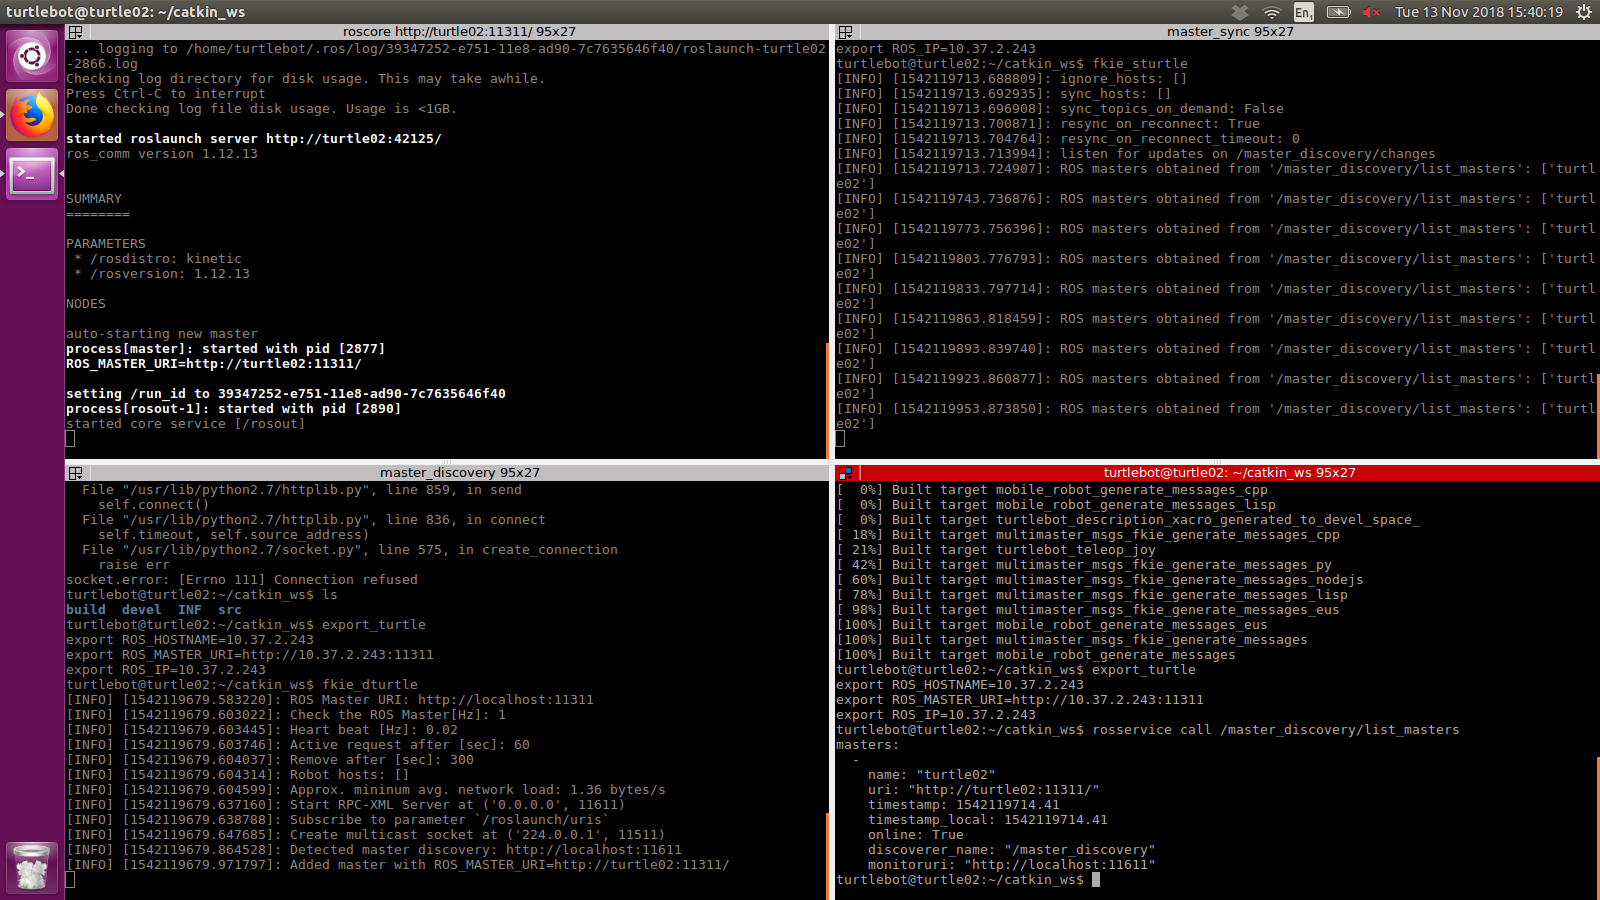
\includegraphics[width=2in]{5.png}
\caption{A view of a successfull setup of the multimaster{\_}fkie.}
\end{center}
\label{fig:mypicture4}
\end{figure}


\end{enumerate}











\end{enumerate}
\section{Conclusion}


Multi-agent system is a topic that has generated a lot interest in the research community. This interest is because a multi-agent systems present a more robust and cheaper solution to a certain tasks that are better performed using several low-cost robots rather than a single one. Multi-agent system can be achieved through many approaches. The approach used in this paper is the one based on the leader-follower premise.
The details of implementation for both simulation as well
as actual experiment is provided which will be useful for
students and practicing engineers alike. These details provide
an insight into the working of each of the these modes of
operation allowing us to identify the strengths and weaknesses
of each one of them.


















%%%%%%%%%%%%%%%%
%%%%%%%%%%%%%%%%%%
%%%%%%%%%%%%%%%%%%%%

\begin{thebibliography}{1}

\bibitem{temp1}
\bibitem{temp2}
\bibitem{temp3}
http://www.ros.org/about-ros/
\bibitem{temp4}
http://wiki.ros.org/turtlebot/Tutorials/indigo
\bibitem{temp5}
https://github.com/Sinchiguano/Multi-agent-system/tree/master/src/multi{\_}agents
\bibitem{temp6}
http://wiki.ros.org/turtlebot
\bibitem{temp7}
http://wiki.ros.org/turtlebot{\_}simulator
\bibitem{temp8}
http://wiki.ros.org/kobuki
\bibitem{temp9}
http://wiki.ros.org/turtlebot{\_}interactions

\bibitem{temp10}
https://github.com/ros/geometry

\bibitem{temp11}
http://wiki.ros.org/ROS/NetworkSetup


\bibitem{temp12}
multimaster FKIE, http://wiki.ros.org/multimaster{\_}fkie
\end{thebibliography}

\end{document}





%
Please ~\ref{fig:mypicture2}

I implemented in the supplied filter.py module as the function called $modified_{\_}accuracy$ which uses the confusion matrix feature to compute TP, FP, TN, FN.

$$macc=\frac{n_{TP}+n_{TN}}{n_{TP}+n_{TN}+10*n_{FP}+n_{FN}}$$